\documentclass[11pt]{article}
\usepackage[margin=1in]{geometry}
\usepackage{amsmath,amssymb}
\usepackage{booktabs,tabularx,array,longtable}
\usepackage{enumitem}
\usepackage{xcolor}
\usepackage[hidelinks]{hyperref}
\usepackage{titlesec}
\usepackage{fancyhdr}
\usepackage{microtype}
\usepackage{lmodern}
\usepackage[T1]{fontenc}
\usepackage{float}
\usepackage{graphicx}
\usepackage{caption}
\usepackage[most]{tcolorbox}
\usepackage{adjustbox}
\usepackage[htt]{hyphenat}
\sloppy

\definecolor{jhublue}{RGB}{0,45,114}
\definecolor{boxgray}{RGB}{244,246,250}
\titleformat{\section}{\large\bfseries\color{jhublue}}{\thesection}{0.6em}{}
\titleformat{\subsection}{\normalsize\bfseries}{\thesubsection}{0.6em}{}
\titleformat{\subsubsection}{\normalsize\itshape}{\thesubsubsection}{0.6em}{}
\setlist{itemsep=2pt,topsep=3pt}
\captionsetup{font=small,labelfont=bf}
\pagestyle{fancy}\fancyhf{}
\cfoot{\small\thepage}
\renewcommand{\headrulewidth}{0.3pt}
\emergencystretch=3em

\newcommand{\PSI}{\mathrm{PSI}}
\newcommand{\file}[1]{\texttt{\small #1}}
\newtcolorbox{summarybox}{colback=boxgray,colframe=jhublue,boxrule=0.6pt,arc=2pt,left=6pt,right=6pt,top=4pt,bottom=4pt,fonttitle=\bfseries,title=Summary}
\newtcolorbox{conceptbox}[1]{colback=white,colframe=jhublue!60,boxrule=0.4pt,arc=2pt,left=6pt,right=6pt,top=3pt,bottom=3pt,fonttitle=\bfseries\small,title={Concept: #1}}
\newtcolorbox{whybox}{colback=boxgray,colframe=gray!50,boxrule=0.4pt,arc=2pt,left=6pt,right=6pt,top=3pt,bottom=3pt}

\lhead{\small Replication of Zhang et al.\ (2026) --- Task 3}
\rhead{\small Sahil, Johns Hopkins University}

\begin{document}

\begin{center}
{\LARGE\bfseries Task 3: Staggered difference-in-differences}\\[6pt]
{\large Does adopting solar policy change bird diversity?}\\[8pt]
Sahil \quad$\cdot$\quad Research Assistant, Johns Hopkins University\\
{\small Prepared for Prof.\ Paul J.\ Ferraro \quad$\cdot$\quad November 2026 \quad$\cdot$\quad All analysis in Stata (StataNow/BE 19.5)}
\end{center}

\begin{summarybox}
\small
\begin{itemize}[leftmargin=12pt]
\item \textbf{Design.} Treatment = the first year a county issues any solar policy (PSI\,$>0$), taken from the full annual policy file. The main sample has 939 counties with measured PSI: 819 adopters in nine cohorts (2015--2023) and 120 never-adopters.
\item \textbf{No evidence that adoption lowers bird diversity.} All four estimators give small, positive, insignificant overall effects: TWFE $+0.032$, Callaway--Sant'Anna $+0.057$, Borusyak--Jaravel--Spiess (BJS) $+0.078$, Sun--Abraham $+0.024$. The most precise heterogeneity-robust estimate, BJS, has SE 0.069 and 95\% CI $-0.058$ to $+0.214$. In the main sample, the only individually significant event-time estimates are \emph{positive}, in the adoption year (about $+0.11$, TWFE and BJS).
\item \textbf{Pre-trends: mixed evidence.} The event-study pre-period estimates are small and individually insignificant (joint tests $p=0.24$ for BJS and $p=0.34$ for TWFE). However, Callaway--Sant'Anna's test of \emph{all} pre-period cohort-year cells rejects parallel trends ($p<0.001$), so the design assumption is not secure.
\item \textbf{Treating the 724 missing-PSI counties as never-treated} (what the paper's coding implies) turns the estimates negative (BJS $-0.087$, SE 0.060; Callaway--Sant'Anna $-0.091$, SE 0.120). But adopters were already falling behind those counties \emph{before} adopting ($-0.17$ at $t=-1$), so this reflects the comparison group, not the policy.
\item \textbf{Caveat.} Binary adoption discards the dose, and the confidence intervals cannot rule out small negative effects.
\end{itemize}
\end{summarybox}

\tableofcontents

%==========================================================================
\section{What Task 3 asks, and why}
Prof.\ Ferraro asked for a \emph{staggered difference-in-differences analysis}, following Baker, Callaway, Cunningham, Goodman-Bacon and Sant'Anna (2025).

\textbf{Why.} Counties start issuing solar policy in different years, a \emph{staggered} rollout. Recent work shows that the standard TWFE regression can be badly biased in this setting when effects vary across cohorts or grow over time. It can even get the sign wrong. Modern staggered-DiD estimators compare each adopting cohort only with counties that have \emph{not yet} adopted. They also produce event studies that show whether adopters and non-adopters were on parallel paths \emph{before} adoption, the key testable implication of the design.

%==========================================================================
\section{Concepts}

\begin{conceptbox}{Difference-in-differences (DiD)}
Compare the change in the outcome for treated units with the change for untreated units over the same period. The untreated change stands in for what would have happened to the treated without treatment. This requires \textbf{parallel trends}: absent treatment, both groups would have changed by the same amount.
\end{conceptbox}

\begin{conceptbox}{Staggered adoption and ``forbidden comparisons''}
When units adopt at different times, TWFE averages every possible two-group, two-period comparison. Some of these use \emph{already-treated} units as controls for later adopters. If effects change over time, those comparisons subtract part of the effect itself, so the TWFE coefficient can be biased or even negative-weighted (Goodman-Bacon 2021).
\end{conceptbox}

\begin{conceptbox}{Group-time ATT (Callaway and Sant'Anna 2021)}
Estimate a separate effect $ATT(g,t)$ for each adoption cohort $g$ in each year $t$. Each one is a clean 2$\times$2 DiD against counties not yet treated at $t$. These are then averaged into an overall ATT or an event study (effect by years since adoption).
\end{conceptbox}

\begin{conceptbox}{Imputation (Borusyak, Jaravel and Spiess 2024)}
Fit the county and time fixed effects using \emph{only untreated observations}. Predict (``impute'') each treated observation's untreated outcome, and average the differences. It uses all clean comparisons efficiently and handles unbalanced panels.
\end{conceptbox}

\begin{conceptbox}{Interaction-weighted event study (Sun and Abraham 2021)}
Estimate cohort-specific event-time effects against a clean control cohort (here, never-treated counties), then average them with weights equal to cohort shares. This avoids the contamination of the standard dynamic TWFE event study.
\end{conceptbox}

\begin{conceptbox}{Event study and pre-trends}
Effects plotted by years relative to adoption. Coefficients \emph{before} adoption should be near zero; if they are not, adopters were already diverging, and parallel trends is doubtful.
\end{conceptbox}

%==========================================================================
\section{From a continuous index to a staggered design}

\subsection{Defining treatment}
The paper's PSI is a continuous annual \emph{flow} (Task 1). A staggered DiD needs a treatment date, so:
\begin{itemize}
\item \textbf{Adoption year $g$} = the first year 2014--2023 in which a county's PSI\,$>0$, taken from \file{PI.dta} for all years, not only the months with bird records.
\item \textbf{Absorbing treatment.} Once a county has issued solar policy it is treated from then on. PSI returns to zero in 15.3\% of post-adoption years, but policies once issued are assumed to persist.
\item \textbf{Already treated in 2014} (838 counties): these have no pre-adoption year, so no DiD comparison is possible and they are dropped.
\end{itemize}

\subsection{Samples}
\begin{itemize}
\item \textbf{Main sample:} counties whose PSI is actually measured. Never-treated = 120 counties in \file{PI.dta} with PSI\,$=0$ in every year.
\item \textbf{Paper-style sample:} additionally treats the 724 counties missing from \file{PI.dta}, almost all urban districts, as never-treated. This is what the authors' ``PSI\,$=0$ if missing'' implies.
\end{itemize}

\begin{table}[H]\centering\small
\caption{Adoption cohorts (counties; \file{tables/3\_1\_cohort\_sizes.csv})}
\begin{adjustbox}{max width=\linewidth}
\begin{tabular}{lrrrrrrrrrr}
\toprule
Cohort & Never & 2015 & 2016 & 2017 & 2018 & 2019 & 2020 & 2021 & 2022 & 2023\\
\midrule
Main sample & 120 & 299 & 85 & 75 & 14 & 68 & 2 & 91 & 30 & 155\\
Paper-style & 844 & 299 & 85 & 75 & 14 & 68 & 2 & 91 & 30 & 155\\
\bottomrule
\end{tabular}
\end{adjustbox}
\end{table}

\subsection{Outcome and time unit}
\begin{itemize}
\item \textbf{TWFE, BJS and SA} use the authors' monthly data and fixed-effect structure: ShannonBD, county and year-month fixed effects, effects by years since adoption, and county-clustered SEs.
\item \textbf{Callaway--Sant'Anna} is defined on a panel of periods. Monthly Shannon is first stripped of month-of-year effects, so that changes in which months were observed do not masquerade as change, and then averaged to county-years (7,984 county-years). The panel is unbalanced. By default \file{csdid} would \emph{balance} it by dropping every county not observed in all ten years, which removes 903 of 939 counties. We therefore use \texttt{bal(pair)}, which balances each 2$\times$2 comparison separately, so every county observed in both years of a comparison is used (3,907 county-years in the main sample, 7,984 in the paper-style sample). Four of the 90 cohort-year cells cannot be estimated because their cohorts are tiny (e.g.\ 2020, two counties), so aggregations exclude them (\texttt{dropmissing}). Callaway--Sant'Anna remains the least precise estimator.
\end{itemize}

%==========================================================================
\section{Workflow}
\begin{table}[H]\centering\small
\caption{Steps in \file{03\_Task3\_Staggered\_DiD/code/}}
\begin{tabularx}{\linewidth}{l>{\raggedright\arraybackslash}X>{\raggedright\arraybackslash}X}
\toprule
Do-file & What and why & Output\\
\midrule
\file{3\_1\_adoption\_timing} & Builds adoption years, cohorts and samples, plus the deseasonalized county-year panel & \file{data/}, \file{tables/3\_1\_cohort\_sizes.csv}\\
\file{3\_2\_twfe\_event\_study} & Conventional static and dynamic TWFE, the benchmark the new estimators correct & \file{tables/3\_2\_twfe.csv}, figure\\
\file{3\_3\_callaway\_santanna} & Group-time ATTs with not-yet-treated controls: unconditional, conditional on urban, paper-style & \file{tables/3\_3\_cs\_*.csv}, figures\\
\file{3\_4\_imputation\_bjs} & Imputation estimator on monthly data, main and paper-style samples & \file{tables/3\_4\_bjs.csv}, figures\\
\file{3\_5\_sun\_abraham} & Interaction-weighted event study, never-treated control cohort & \file{tables/3\_5\_sun\_abraham.csv}, figure\\
\bottomrule
\end{tabularx}
\end{table}

%==========================================================================
\section{Results}

\subsection{Overall effects}
\begin{table}[H]\centering\small
\caption{Average effect of adopting solar policy on Shannon diversity}\label{tab:att}
\begin{adjustbox}{max width=\linewidth}
\begin{tabular}{llccl}
\toprule
Estimator & Sample & ATT & SE & Notes\\
\midrule
TWFE, static (post-adoption dummy) & Main & $+0.032$ & 0.041 & 12,667 county-months, 853 counties\\
Callaway--Sant'Anna & Main & $+0.057$ & 0.143 & not-yet-treated controls; 3,907 county-years\\
Callaway--Sant'Anna, conditional on urban & Main & $+0.057$ & 0.141 & doubly robust\\
\textbf{Borusyak--Jaravel--Spiess} & \textbf{Main} & $\mathbf{+0.078}$ & \textbf{0.069} & county + year FE$^\dagger$\\
Sun--Abraham (mean of years 0--5) & Main & $+0.024$ & 0.089 & never-treated controls\\
\midrule
Callaway--Sant'Anna & Paper-style & $-0.091$ & 0.120 & 7,984 county-years\\
Borusyak--Jaravel--Spiess & Paper-style & $-0.087$ & 0.060 & county + year-month FE\\
\bottomrule
\end{tabular}
\end{adjustbox}
\par\smallskip\footnotesize $^\dagger$In the main sample, year-month effects could not be estimated from untreated observations alone, so BJS falls back to county + year effects. Observations with no untreated counterpart in their county or month were dropped before imputing (3,698).
\end{table}

\begin{whybox}\small
\textbf{Reading Table~\ref{tab:att}.} Among counties whose policy is actually measured, no estimator finds that adopting solar policy lowers bird diversity; every overall point estimate is positive. The most precise heterogeneity-robust estimate (BJS) rules out declines larger than about 0.06 Shannon units, about 6\% of a standard deviation (SD 0.98). It cannot rule out a small decline such as the $-0.034$ from the binary ``any PSI$>$0'' TWFE check in Task 1 (Section 7, Panel B). Only when the missing-PSI urban districts are added as ``never-treated'' do the estimates turn negative, and the event studies below show why.
\end{whybox}

\subsection{Event studies}
\begin{figure}[H]\centering
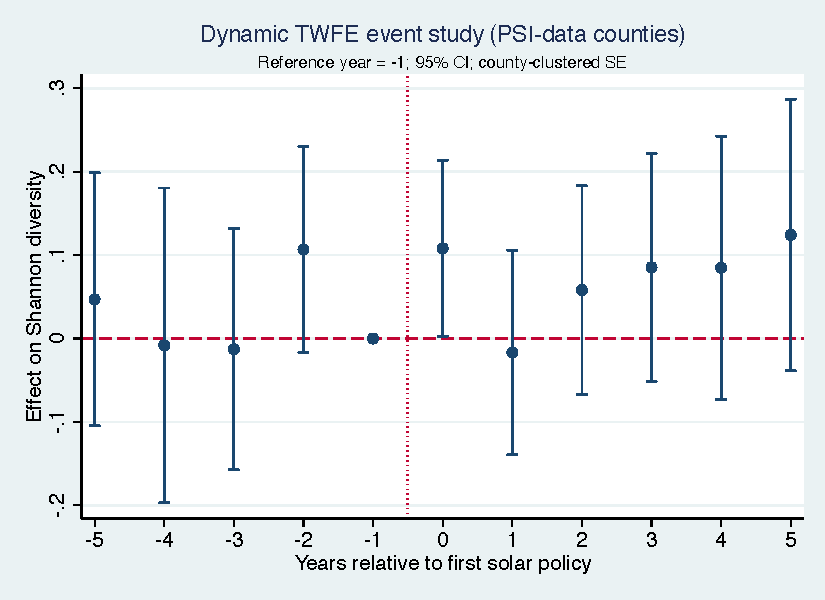
\includegraphics[width=0.49\linewidth]{../figures/3_2_event_study_twfe.pdf}\hfill
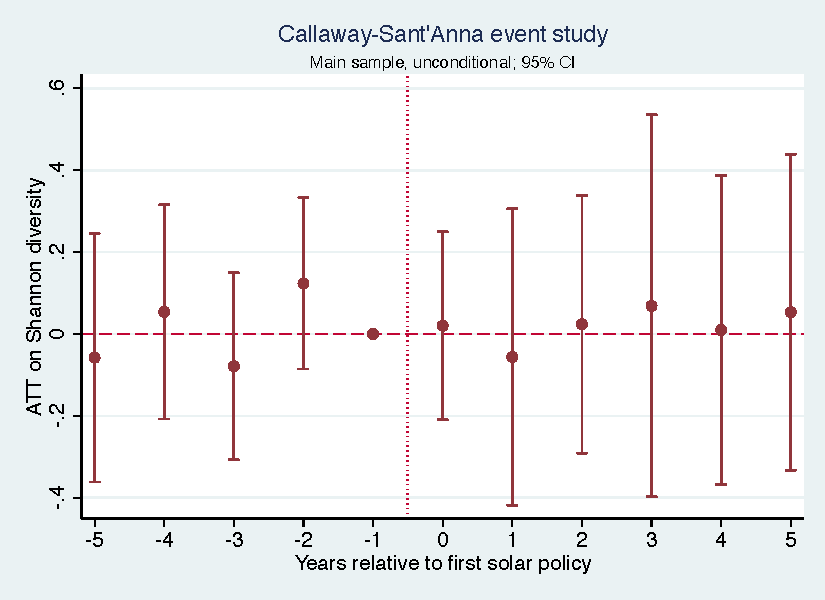
\includegraphics[width=0.49\linewidth]{../figures/3_3_event_study_cs_1.pdf}\\[4pt]
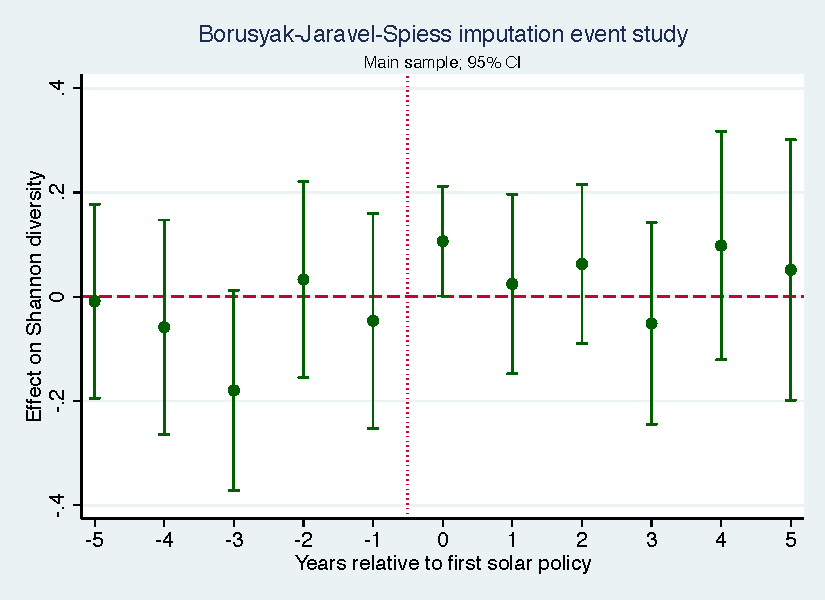
\includegraphics[width=0.49\linewidth]{../figures/3_4_event_study_bjs_1.pdf}\hfill
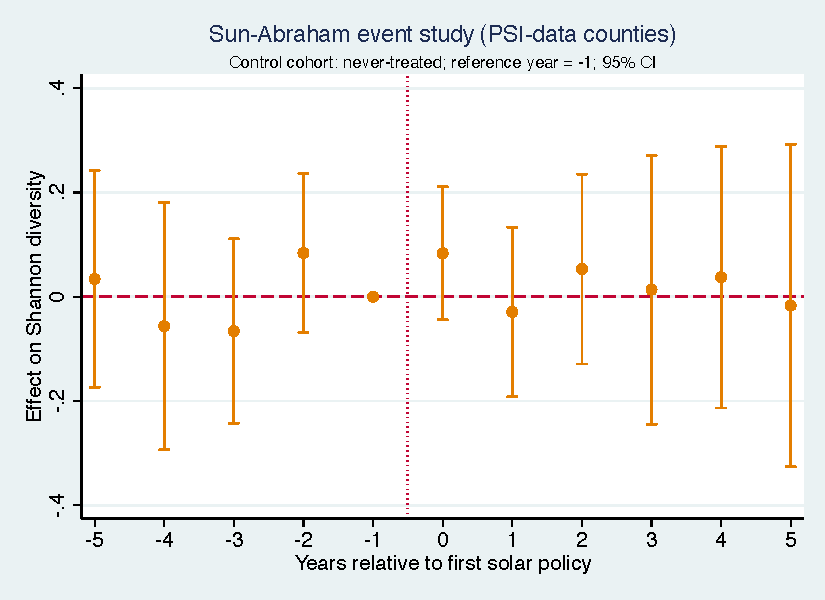
\includegraphics[width=0.49\linewidth]{../figures/3_5_event_study_sa.pdf}
\caption{Main sample (measured-PSI counties). Effects by years relative to first solar policy, 95\% CIs. Top left: conventional dynamic TWFE. Top right: Callaway--Sant'Anna. Bottom left: BJS imputation. Bottom right: Sun--Abraham. Pre-adoption coefficients scatter around zero (joint tests $p=0.34$ TWFE, $p=0.24$ BJS), and no post-adoption decline appears. Callaway--Sant'Anna's own test across all pre-period cohort-year cells nonetheless rejects parallel trends ($p<0.001$); see Section 6.}
\end{figure}

\begin{figure}[H]\centering
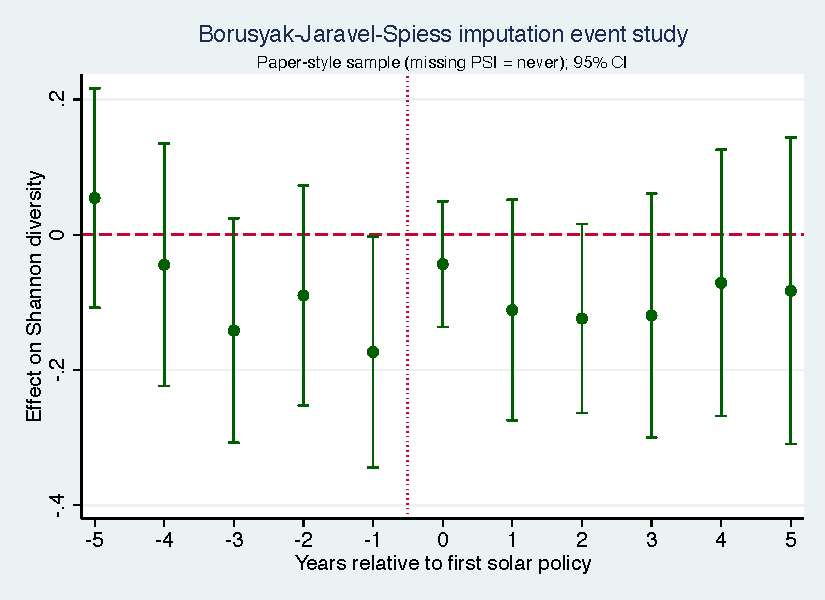
\includegraphics[width=0.49\linewidth]{../figures/3_4_event_study_bjs_2.pdf}\hfill
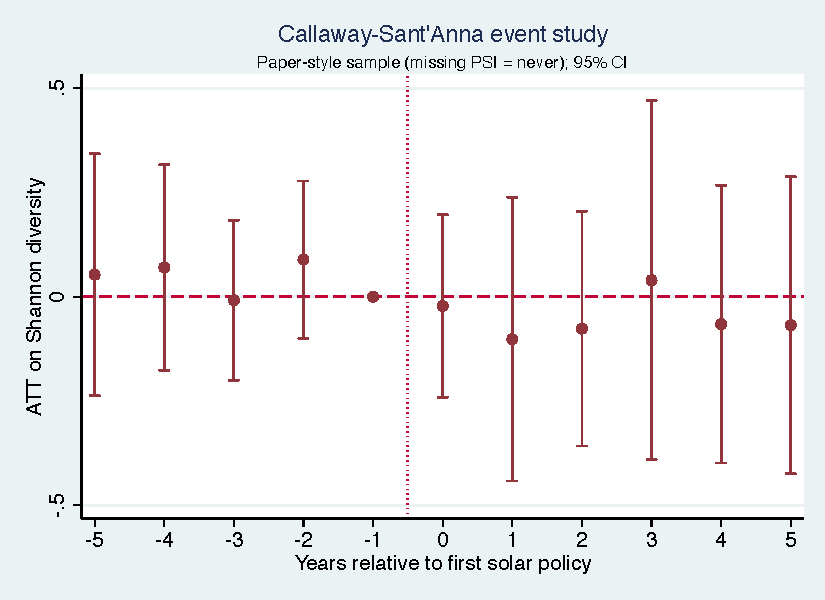
\includegraphics[width=0.49\linewidth]{../figures/3_3_event_study_cs_3.pdf}
\caption{Paper-style sample (missing-PSI counties treated as never-treated). Left: BJS. Right: Callaway--Sant'Anna. In the BJS plot adopters are already below the imputed counterfactual \emph{before} adoption ($-0.17$, SE 0.09, at $t=-1$; joint pre-trend $p=0.14$), and post-adoption estimates continue that path. The negative ``effect'' reflects pre-existing divergence from the mostly urban comparison group.}
\end{figure}

\begin{table}[H]\centering\small
\caption{Selected event-time estimates (SE)}
\begin{adjustbox}{max width=\linewidth}
\begin{tabular}{lcccc}
\toprule
Years since adoption & TWFE & BJS (main) & SA & BJS (paper-style)\\
\midrule
$-3$ & $-0.013$ (0.074) & $-0.179$ (0.098) & $-0.066$ (0.090) & $-0.142$ (0.085)\\
$-2$ & $+0.107$ (0.063) & $+0.033$ (0.096) & $+0.084$ (0.078) & $-0.090$ (0.083)\\
$-1$ & 0 (ref.) & $-0.046$ (0.105) & 0 (ref.) & $-0.173$ (0.087)\\
$0$ & $+0.108$ (0.054) & $+0.107$ (0.054) & $+0.084$ (0.065) & $-0.043$ (0.047)\\
$1$ & $-0.017$ (0.062) & $+0.025$ (0.088) & $-0.029$ (0.083) & $-0.111$ (0.083)\\
$2$ & $+0.058$ (0.064) & $+0.063$ (0.078) & $+0.053$ (0.093) & $-0.124$ (0.071)\\
$3$ & $+0.085$ (0.070) & $-0.051$ (0.099) & $+0.014$ (0.131) & $-0.119$ (0.092)\\
\bottomrule
\end{tabular}
\end{adjustbox}
\par\smallskip\footnotesize TWFE and SA use $t=-1$ as the reference; BJS pre-period coefficients compare each pre-period with the imputed counterfactual, so BJS has no reference year.
\end{table}

%==========================================================================
\section{Interpretation and limitations}
\begin{enumerate}
\item \textbf{Consistent with Tasks 1--2.} The paper's negative association disappears once comparisons are restricted to counties whose policy status is actually measured. The same urban comparison group that drives the TWFE result also produces the only negative DiD estimates here, and those come with a visible pre-trend.
\item \textbf{Parallel trends is not secure.} The aggregated pre-period estimates are small, but Callaway--Sant'Anna's joint pre-test over all individual pre-period cells rejects ($p<0.001$) in every specification. These cells reach up to nine years before adoption, and some rest on very few counties, which may drive the rejection; this has not been verified. Either way, the DiD results should be read as ``no evidence of a negative effect'' rather than as a precise null.
\item \textbf{Binary adoption loses the dose.} The paper's claim is about policy \emph{intensity}. A continuous-treatment DiD (Callaway, Goodman-Bacon and Sant'Anna 2024; Baker et al.\ 2025, App.\ A.2) is the natural extension.
\item \textbf{Absorbing treatment} is an assumption. PSI returns to zero in 15\% of post-adoption years.
\item \textbf{Early adopters are excluded.} The 838 counties already treated in 2014 cannot be used, so the results describe later adopters only.
\item \textbf{Precision.} Callaway--Sant'Anna works on county-year averages of an unbalanced panel and is the least precise. BJS uses the monthly data and is more precise, but needed county + year (not year-month) effects in the main sample.
\item \textbf{Selection on observation} (Task 1) still applies: outcomes exist only where people went birding.
\end{enumerate}

\section{How to reproduce}
In Stata, type
\begin{quote}\small\texttt{do ".../03\_Task3\_Staggered\_DiD/code/3\_0\_run\_task3.do"}\end{quote} This needs Task 1's analysis sample, and installs \file{csdid}, \file{drdid}, \file{did\_imputation}, \file{eventstudyinteract} and \file{avar} if they are missing. Callaway--Sant'Anna SEs use a multiplier bootstrap with a fixed seed (20261107).

\section*{References}
{\small
\begin{itemize}[leftmargin=12pt,label={}]
\item Baker, A., Callaway, B., Cunningham, S., Goodman-Bacon, A.\ and Sant'Anna, P.\ H.\ C.\ (2025). Difference-in-differences designs: a practitioner's guide. \textit{Journal of Economic Literature}, 64(2), 498--557 (preprint arXiv:2503.13323).
\item Borusyak, K., Jaravel, X.\ and Spiess, J.\ (2024). Revisiting event-study designs: robust and efficient estimation. \textit{Review of Economic Studies}, 91(6), 3253--3285.
\item Callaway, B.\ and Sant'Anna, P.\ H.\ C.\ (2021). Difference-in-differences with multiple time periods. \textit{Journal of Econometrics}, 225(2), 200--230.
\item Callaway, B., Goodman-Bacon, A.\ and Sant'Anna, P.\ H.\ C.\ (2024). Difference-in-differences with a continuous treatment. NBER Working Paper 32117.
\item Goodman-Bacon, A.\ (2021). Difference-in-differences with variation in treatment timing. \textit{Journal of Econometrics}, 225(2), 254--277.
\item Sun, L.\ and Abraham, S.\ (2021). Estimating dynamic treatment effects in event studies with heterogeneous treatment effects. \textit{Journal of Econometrics}, 225(2), 175--199.
\item Zhang, H.\ et al.\ (2026). China's solar expansion policy reduces bird diversity. \textit{Science}, 393, 831.
\end{itemize}}

\end{document}
